\documentclass{article}

\usepackage{graphicx}
\usepackage{tikz}
\usepackage{tikzsymbols}
\usetikzlibrary{calc,patterns,shapes.geometric}
\pagestyle{empty}
\usepackage[margin=0pt]{geometry}
\geometry{papersize={14in,12in}}

\def\centerarc[#1](#2)(#3:#4:#5){\draw[#1] ($(#2)+({#5*cos(#3)},{#5*sin(#3)})$) arc (#3:#4:#5);}

\begin{document}
	\begin{figure}
		\centering
		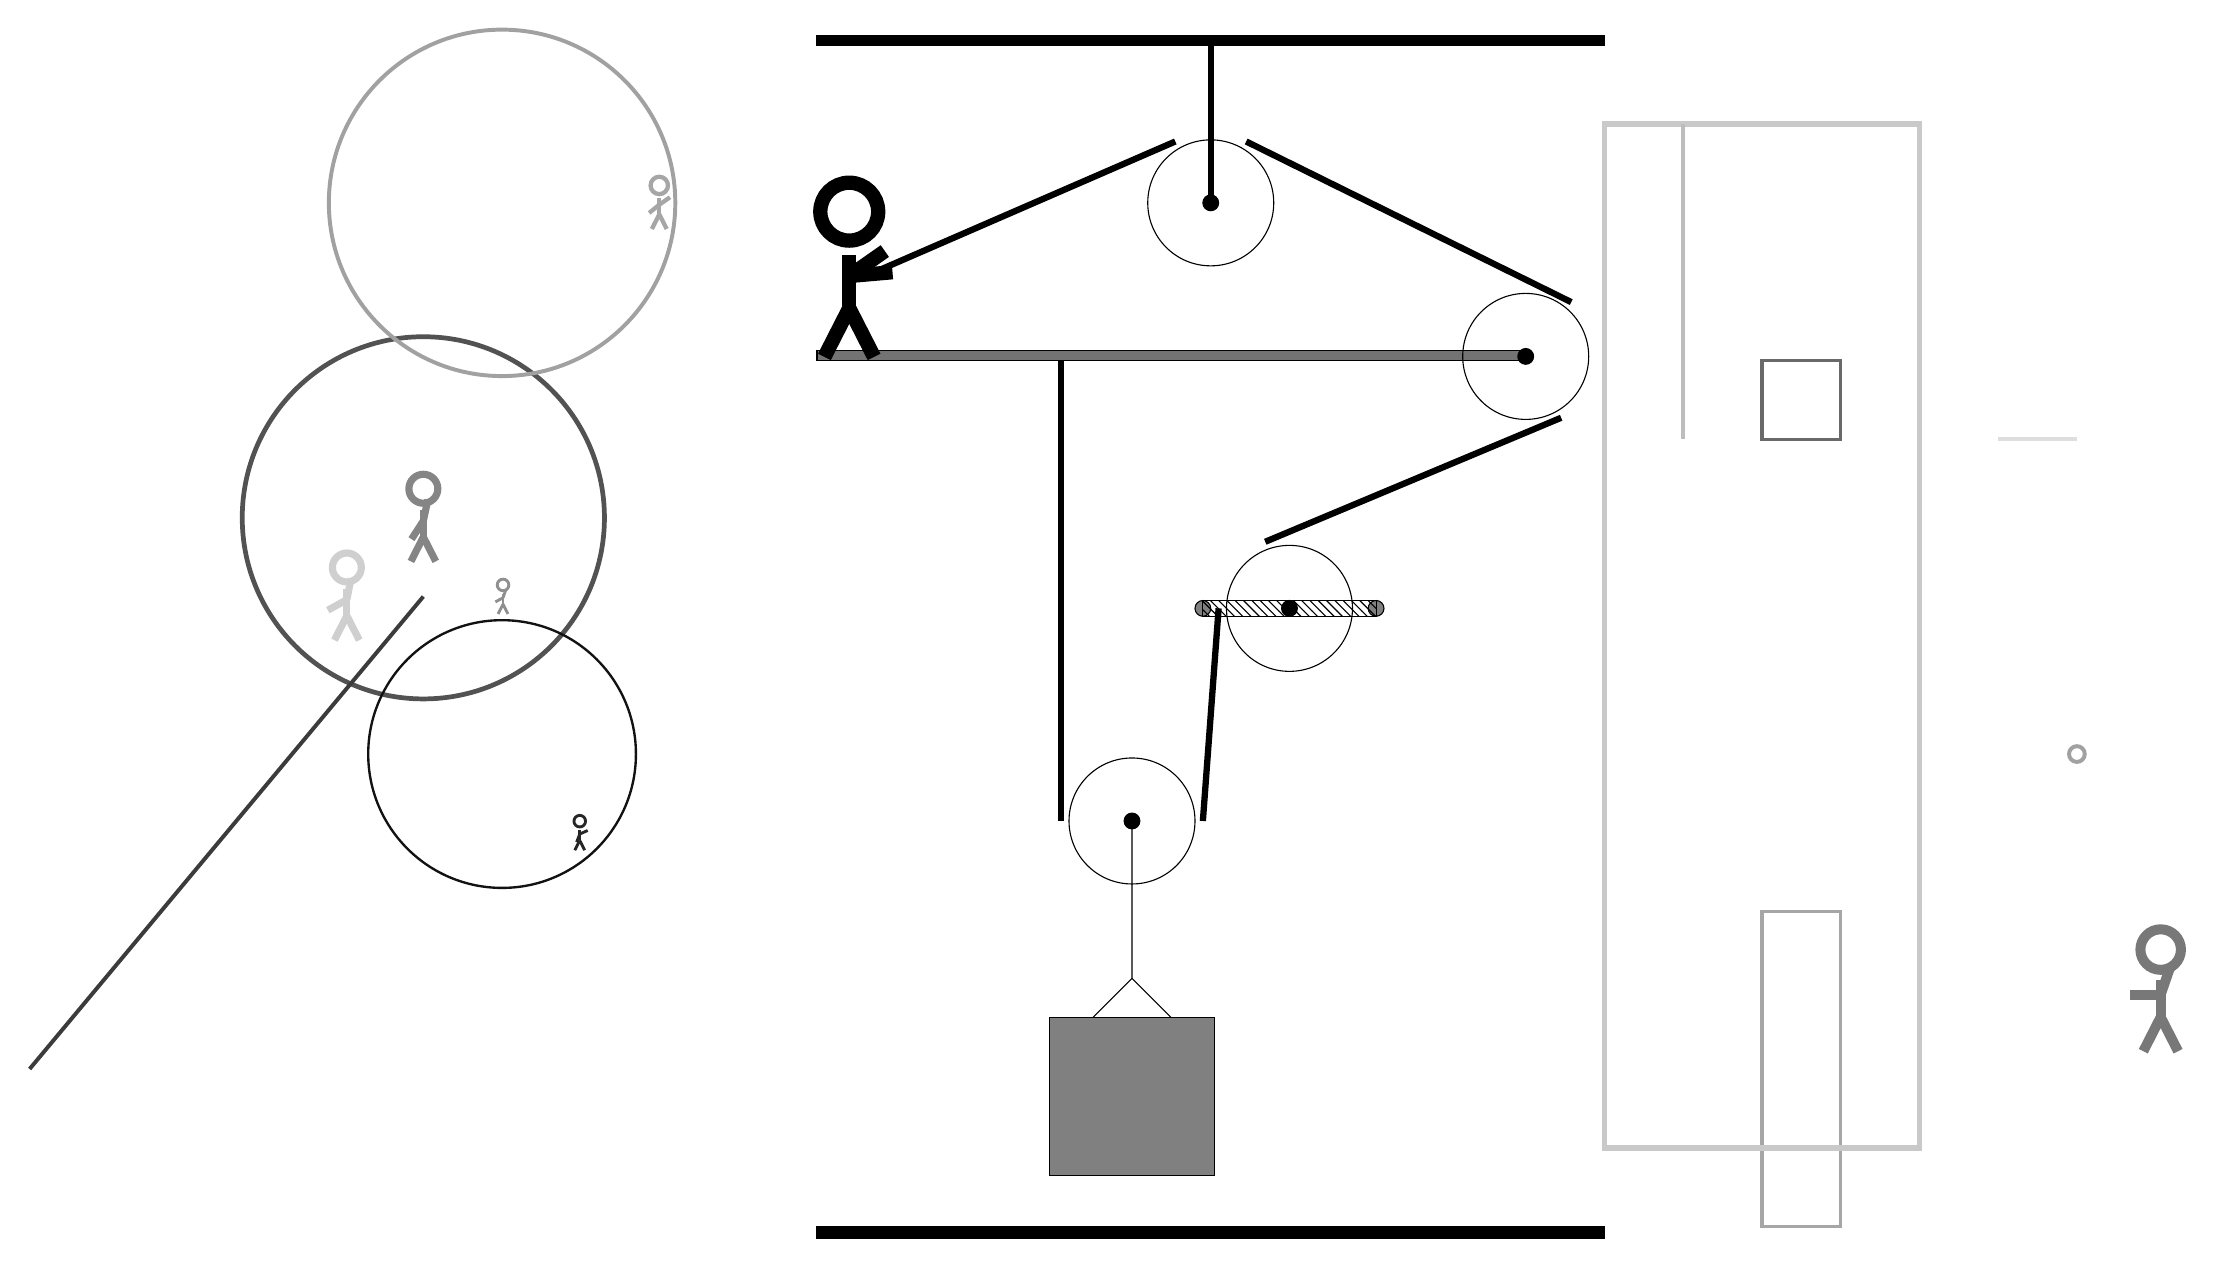
\begin{tikzpicture}
			%%%%% START %%%%%
			
			\draw[fill=black] (-2, 13) rectangle (8, 13.125);
			
			\draw[fill=black!55] (-2, 9) rectangle (7, 9.125);
			
			\draw (2, 3.15) circle (0.8);
			\draw[fill=black] (2, 3.15) circle (0.1);
			
			\draw (7, 9.05) circle (0.8);
			\draw[fill=black] (7, 9.05) circle (0.1);
			
			\draw[fill=white](4, 5.85) circle (0.8);
			\draw[fill=black] (4, 5.85) circle (0.1);
			\draw[fill=black!50] (2.9, 5.85) circle (0.1);
			\draw[fill=black!50] (5.1, 5.85) circle (0.1);
			\draw[pattern=north west lines, pattern color=black] (2.9, 5.95) rectangle (5.1, 5.75);
			
			\draw (3, 11) circle (0.8);
			\draw[fill=black] (3, 11) circle (0.1);
			\draw[line width=0.8mm] (3, 11) -- (3, 13);
			
			\draw (2, 3.15) -- (2, 1.15) -- (1.5, 0.65) -- (2.5, 0.65) -- (2, 1.15);
			\draw[fill=black!50] (0.95, 0.65) rectangle (3.05, -1.35);
			
			\draw[line width=0.8mm] (1.1, 9) -- (1.1, 3.15);
			\centerarc[line width=0.8mm](2, 3.15)(180:360:0.9);
			\draw[line width=0.8mm](2.9, 3.15) -- (3.1, 5.85);
			\centerarc[line width=0.8mm](4, 5.85)(110:180:0.9);
			\draw[line width=0.8mm](3.6922, 6.6957) -- (7.45, 8.2706);
			\centerarc[line width=0.8mm](7, 9.05)(-60:50:0.9);
			\draw[line width=0.8mm](7.5785, 9.7394) -- (3.45, 11.7794);
			\centerarc[line width=0.8mm](3, 11)(60:120:0.9);
			\draw[line width=0.8mm](2.55, 11.7794) -- (-1.2, 10.15);
			
			\node at (-1.5, 10.15) {\Strichmaxerl[10][-175][35]};
			
			\node[line width=0.5mm, color=black!44] at (-6, 6) {\Strichmaxerl[2][28][71]};
			
			\node[line width=0.3mm, color=black!48] at (-7, 7) {\Strichmaxerl[5][57][78]};
			\draw [line width=0.6mm, color=black!68](-7, 7) circle (2.3);
			\draw[line width=0.4mm, color=black!35] (10, 2) rectangle (11, -2);
			\draw[line width=0.7mm, color=black!21] (8, -1) rectangle (12, 12);
			\draw [line width=0.5mm, color=black!37](14, 4) circle (0.1);
			
			\draw[line width=0.4mm, color=black!59] (10, 9) rectangle (11, 8);
			\draw[line width=0.5mm, color=black!26](9, 12) -- (9, 8);
			\draw [line width=0.3mm, color=black!93](-6, 4) circle (1.7);
			\node[line width=0.3mm, color=black!19] at (-8, 6) {\Strichmaxerl[5][29][79]};
			\draw[line width=0.5mm, color=black!13](13, 8) -- (14, 8);
			\node[line width=0.7mm, color=black!85] at (-5, 3) {\Strichmaxerl[2][69][24]};
			\draw[line width=0.5mm, color=black!77](-7, 6) -- (-12, 0);
			
			\node[line width=0.4mm, color=black!53] at (15, 1) {\Strichmaxerl[7][0][71]};
			\draw [line width=0.5mm, color=black!37](-6, 11) circle (2.2);
			\node[line width=0.4mm, color=black!35] at (-4, 11) {\Strichmaxerl[3][39][35]};
			
			\draw[fill=black] (-2, -2) rectangle (8, -2.15);
			
			%%%%% END %%%%%
		\end{tikzpicture}
	\end{figure}	
\end{document}